\documentclass[a4paper,10pt]{article}
\usepackage[utf8x]{inputenc}
\usepackage{graphicx}
\usepackage{pgf}
\pgfdeclareimage[height=1cm]{myimage}{p1_q1.png}
\usepackage{listings}
\usepackage[portuguese]{babel}

%----------------- CONFIGURAÇÃO PARA OS COMANDOS -----------------------

\lstset
{
  basicstyle = \footnotesize, 		% Tamanho da fonte do código
  %numbers = left, 			% Posição da numeração das linhas
  %numberstyle = \tiny\color{blue}, 	% Estilo da numeração de linhas
  %stepnumber = 1, 			% Numeração das linhas ocorre a cada quantas linhas?
  %numbersep = 10pt, 			% Distância entre a numeração das linhas e o código
  backgroundcolor = \color{white}, 	% Cor de fundo
  showspaces = false, 			% Exibe espaços com um sublinhado
  showstringspaces = false, 		% Sublinha espaços em Strings
  showtabs = false, 			% Exibe tabulação com um sublinhado
  frame = single, 			% Envolve o código com uma moldura, pode ser single ou trBL
  rulecolor = \color{black}, 		% Cor da moldura
  tabsize = 2, 				% Configura tabulação em x espaços
  captionpos = b, 			% Posição do título pode ser t (top) ou b (bottom)
  breaklines = true, 			% Configura quebra de linha automática
  breakatwhitespace= false, 		% Configura quebra de linha
  title = \lstname, 			% Exibe o nome do arquivo incluido
  %caption = \lstname, % Também é possível usar caption no lugar de title
  keywordstyle = \color{blue}, 		% Estilo das palavras chaves
  commentstyle = \color{dkgreen}, 	% Estilo dos Comentários
  stringstyle = \color{mauve}, 		% Estilo de Strings
  escapeinside = {\%*}{*)}, 		% Permite adicionar comandos LaTeX dentro do seu código
  morekeywords     ={*,...} 		% Se quiser adicionar mais palavras-chave
}

%------------------------------------------------------------------------
%-------------------------------- CAPA ----------------------------------
%------------------------------------------------------------------------

\title{
  Programação Orientada a Objetos\\
  Prof. Fábio Kon\\ ~\\
  \textbf{Sistema Petrolimpa}
}

\author{
  Leonardo Macedo (8536065)\\
  Rodrigo Siqueira (9868770)\\
}

%------------------------------------------------------------------------
%----------------------- SUMÁRIO E DEMAIS ITENS -------------------------
%------------------------------------------------------------------------

\begin{document}
\maketitle
\titlepage

\tableofcontents
\newpage

%------------------------------------------------------------------------
%----------------------------- Visão Geral ------------------------------
%------------------------------------------------------------------------

\section{Visão Geral: Especificação do Sistema}

Na disciplina de \emph{Programação Orientada a Objetos} (MAC0441), ministrada no IME
pelo professor Fábio Kon, foi lançada a tarefa de modelar um sistema para uma
petrolífera com o objetivo de exercitarmos a criação de três diagramas UML. A seguinte
especificação foi fornecida: ~\\

\emph{Você foi contratado por uma grande empresa petrolífera para projetar um
sistema de combate à corrupção interna.} \par

\emph{O sistema deve executar de forma distribuída nos 5 escritórios da empresa
espalhados pelo país, coletando dados dos 1000 postos de gasolina, 20
plataformas de petróleo, 30 centros de distribuição de combustível e 10
refinarias. Não há um único ponto de centralização do sistema, os 5 escritórios
são independentes.} \par

\emph{O sistema utilizará um motor de inferência (utilizando técnicas de
mineração de dados e IA para localizar suspeitas de fraudes que serão postadas
publicamente, diariamente no web site da empresa).} \par

\emph{Cada compra da empresa (que acontecem a uma taxa de milhares por dia,
espalhadas pelo país) pode ser com licitação ou dispensa de licitação. Além
disso, cada compra pode ser de serviços, de equipamentos permanentes ou de
insumos. Finalmente, cada compra pode ser via importação ou no mercado interno.
Para cada tipo diferente de compra, os algoritmos de detecção de fraudes são
diferentes, i.e., personalizados para cada caso. Além disso, há algoritmos
próprios para detectar fraudes analisando-se a totalização dos gastos de cada
unidade (posto, plataforma, centro de distribuição ou refinaria).} \par

\emph{Cada compra deve ser analisada por exatamente 3 escritórios diferentes.} \par

\subsection{Abordagem Utilizada}

Os principais pontos que encontramos no texto estão listados abaixo. Optamos, para
certos casos, em inferir informações da especificação: por exemplo, que tipo de dado
seria relevante para coletar das diferentes fontes.

\begin{enumerate}
  \item Existem 5 escritórios da empresa em locais diferentes;
  \item Os 5 escritórios devem ser independentes;
  \item Os dados são coletados das seguintes fontes:
    \begin{itemize}
      \item 1000 postos de gasolina;
      \item 20 plataformas de petróleo;
      \item 30 centros de distribuição;
      \item 10 refinarias.
    \end{itemize}
  \item O sistema utilizará um motor de inferência para minerar dados e aplicar
        algoritmos de IA;
  \item As compras são subdividas em diferentes categorias:
      \begin{itemize}
        \item Forma da compra: Licitação ou dispensa de licitação;
        \item Tipo da compra: Serviços, equipamentos permanentes ou insumos;
        \item Local da compra: Importação ou no mercado interno.
      \end{itemize}
  \item Para cada tipo de compra, algoritmos diferentes de detecção de fraude
        podem ser usados;
  \item Cada compra é analisada por 3 escritórios diferentes;
  \item O sistema posta diariamente no site da empresa qualquer suspeita de
        fraude.
\end{enumerate}

Em vista dos requisitos levantados, além do obrigatório Diagrama de Implantação,
optamos pelos dois seguintes diagramas:

\begin{itemize}
  \item \textbf{Diagrama de Caso de Uso}: Escolhido pela simplicidade e por mostrar
        uma visão de alto nível do sistema, mostrando as ações que um escritório
        pode realizar.
  \item \textbf{Diagrama de Classes}: Apresenta características e relações entre os
        diferentes componentes do sistema, dividindo-os em classes e pacotes.
\end{itemize}

\newpage

%------------------------------------------------------------------------
%------------------------ Diagrama de Caso de Uso -----------------------
%------------------------------------------------------------------------

\section{Diagrama de Caso de Uso}

Veja a \emph{Figura \ref{uc}} com a modelagem do Diagrama de Caso de Uso para o
Sistema Petrolimpa.

\begin{figure}[ht]
  \centering
  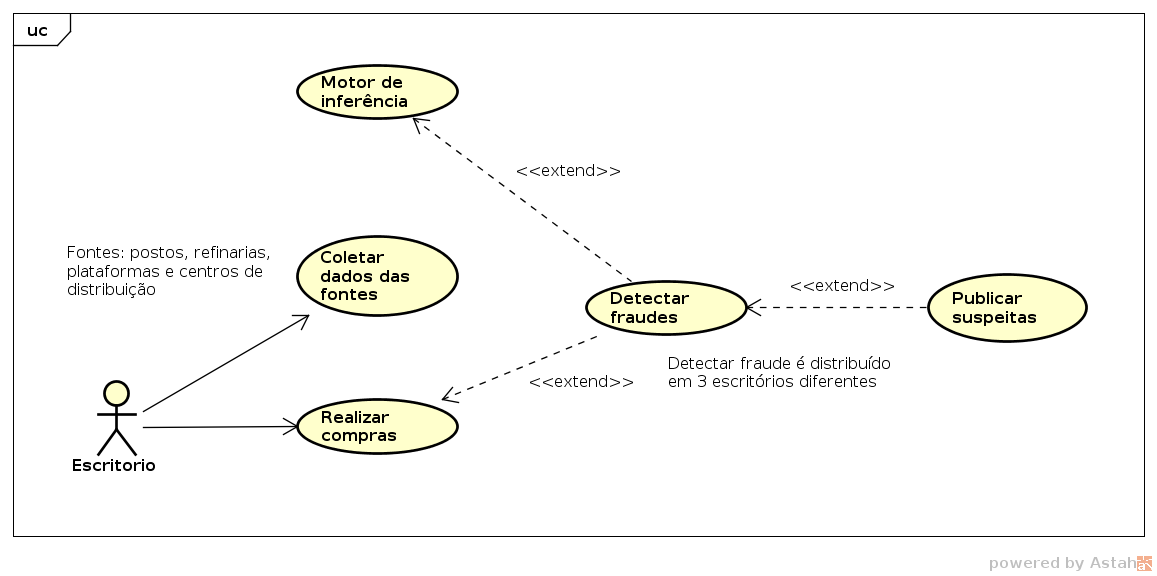
\includegraphics[width=1\textwidth, keepaspectratio=true]{images/uc.png}
  \caption {Diagrama de Caso de Uso}
  \label {uc}
\end{figure}

Segue abaixo uma explicação para cada caso de uso:

\begin{itemize}
  \item \emph{Realizar compras:} Engloba todas as propriedades envolvidas numa compra.
        Na sessão anterior, descrevemos as diferentes formas em que este processo pode
        ocorrer. Este caso de uso possui destaque no sistema, relacionando-se com
        outros módulos.
  \item \emph{Coletar dados da fonte:} Conforme a especificação, o sistema possui
        diferentes fontes que fornecem diversos dados de compra. Neste sentido,
        este caso de uso visa a descrever a forma como tais informações são coletadas
        e mineradas.
  \item \emph{Motor de inferência:} O motor de inferência possui os algoritmos de
        mineração e IA, sendo parte do módulo de detecção de fraudes.
  \item \emph{Detectar fraudes:} A detecção é feita sobre a compra, utilizando-se o
        motor de inferência.
  \item \emph{Publicar suspeitas:} Caso uma fraude seja detectada, ocorre uma
        publicação no website da empresa, apresentando-se os dados analisados.
\end{itemize}

%------------------------------------------------------------------------
%-------------------------- Diagrama de Classes -------------------------
%------------------------------------------------------------------------

\newpage
\section{Diagrama de Classes}

Procuramos abstrair bastante a modelagem de classes, deixando espaços para expansões
no sistema com o menor impacto possível. Em outras palavras, identificamos pontos de
alteração em potencial no sistema e isolamos eles. Para isto, aplicamos várias
técnicas de Orientação a Objetos e alguns padrões de projetos simples. \par

Veja a \emph{Figura \ref{dc}} contendo o Diagrama de Classes completo do projeto
(recomendamos dar "zoom" neste arquivo para visualizar com maior detalhe).

\begin{figure}[ht]
  \centering
  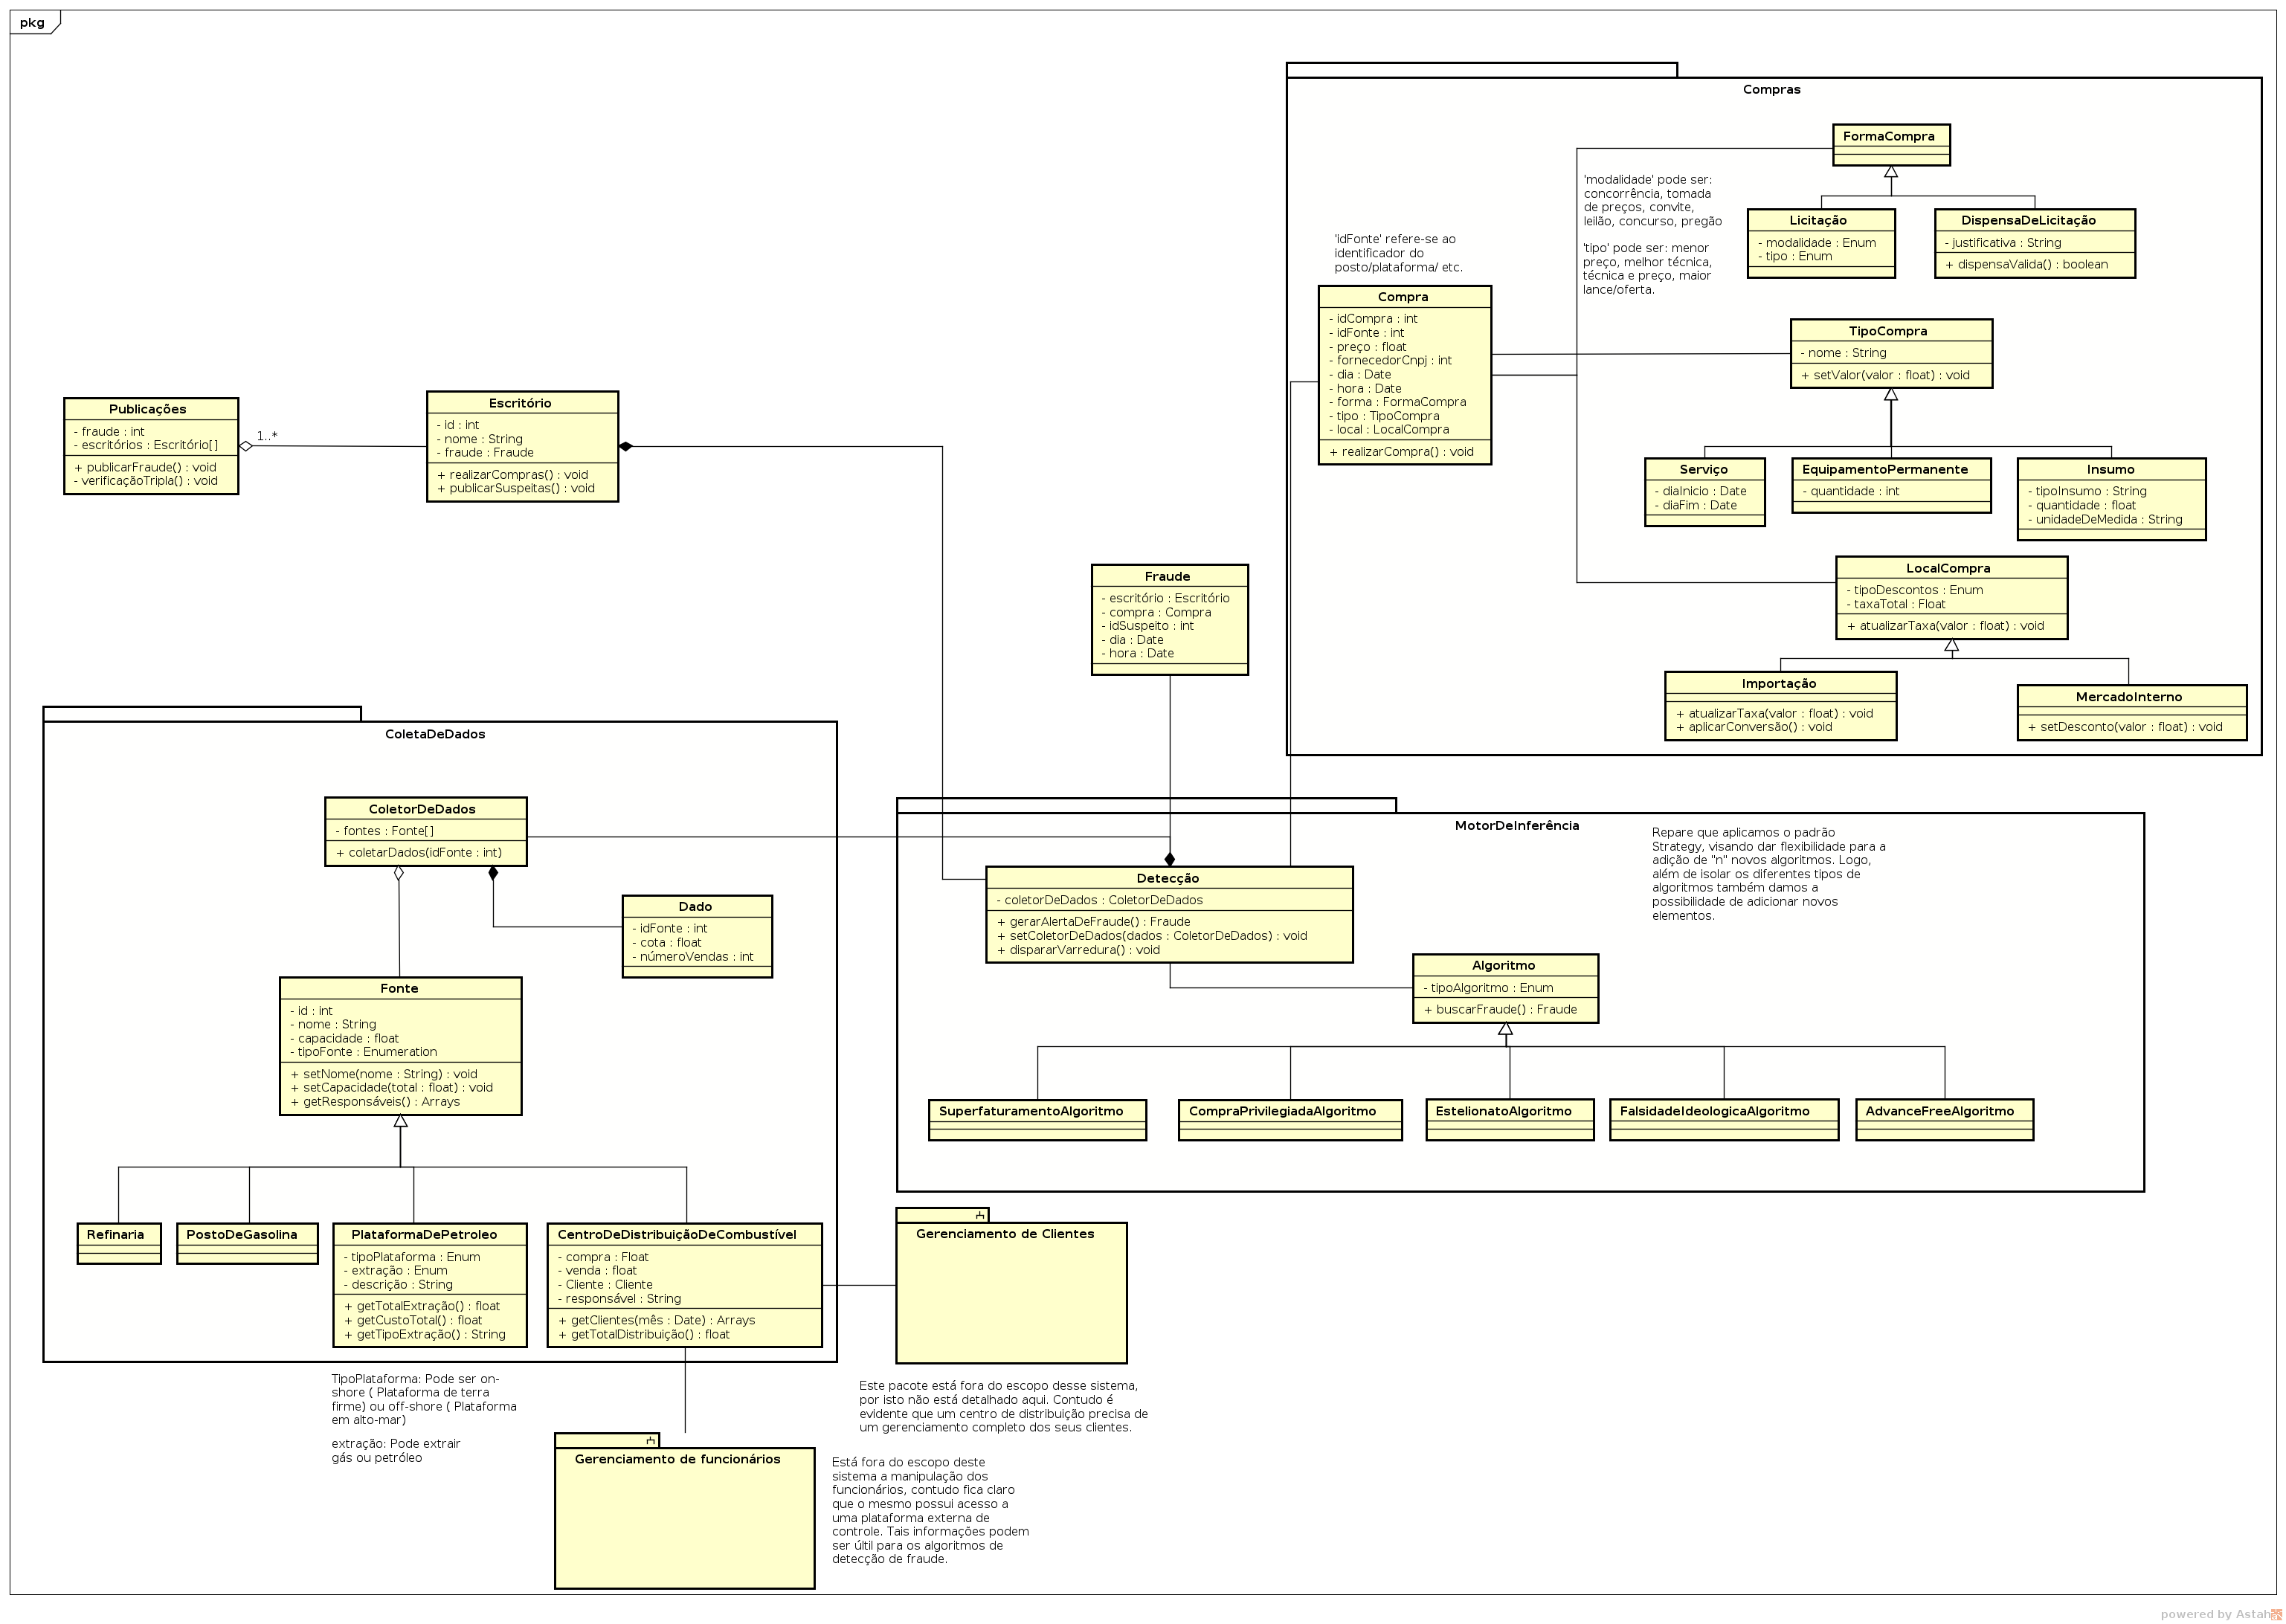
\includegraphics[width=1.2\textwidth, keepaspectratio=true]{images/classes.png}
  \caption {Diagrama de Classes completo}
  \label {dc}
\end{figure}

No canto superior esquerdo está a classe \emph{Escritório}, responsável por executar
o motor de inferência e enviar informações de uma compra para outros dois
escritórios analisarem. A publicação de uma fraude é feita em outra classe,
\emph{Publicações}, para melhor organização do sistema.

\subsection{Módulo de Coleta de Dados}

Para facilitar a compreensão, explicaremos separadamente cada módulo do diagrama.
Começaremos pelo módulo de coleta de dados, responsável por realizar a aquisição de
dados das diferentes fontes do sistema. Veja a \emph{Figura \ref{coleta}} e note que
os diferentes tipos de fontes estão modelados, com cada um fornecendo uma gama
diferente de informações (realizamos uma pesquisa rápida para encontrar dados
interessantes para armazenar). \par

O sistema foi flexibilizado por meio de uma interface comum, que permite a adição de
novas fontes simplesmente extendendo a classe mais abstrata. Há também uma classe
mais externa, chamada \emph{ColetorDeDados}, capaz de juntar as diversas informações e
produzir instâncias do tipo Dado para o algoritmo de detecção.

\begin{figure}[ht]
  \centering
  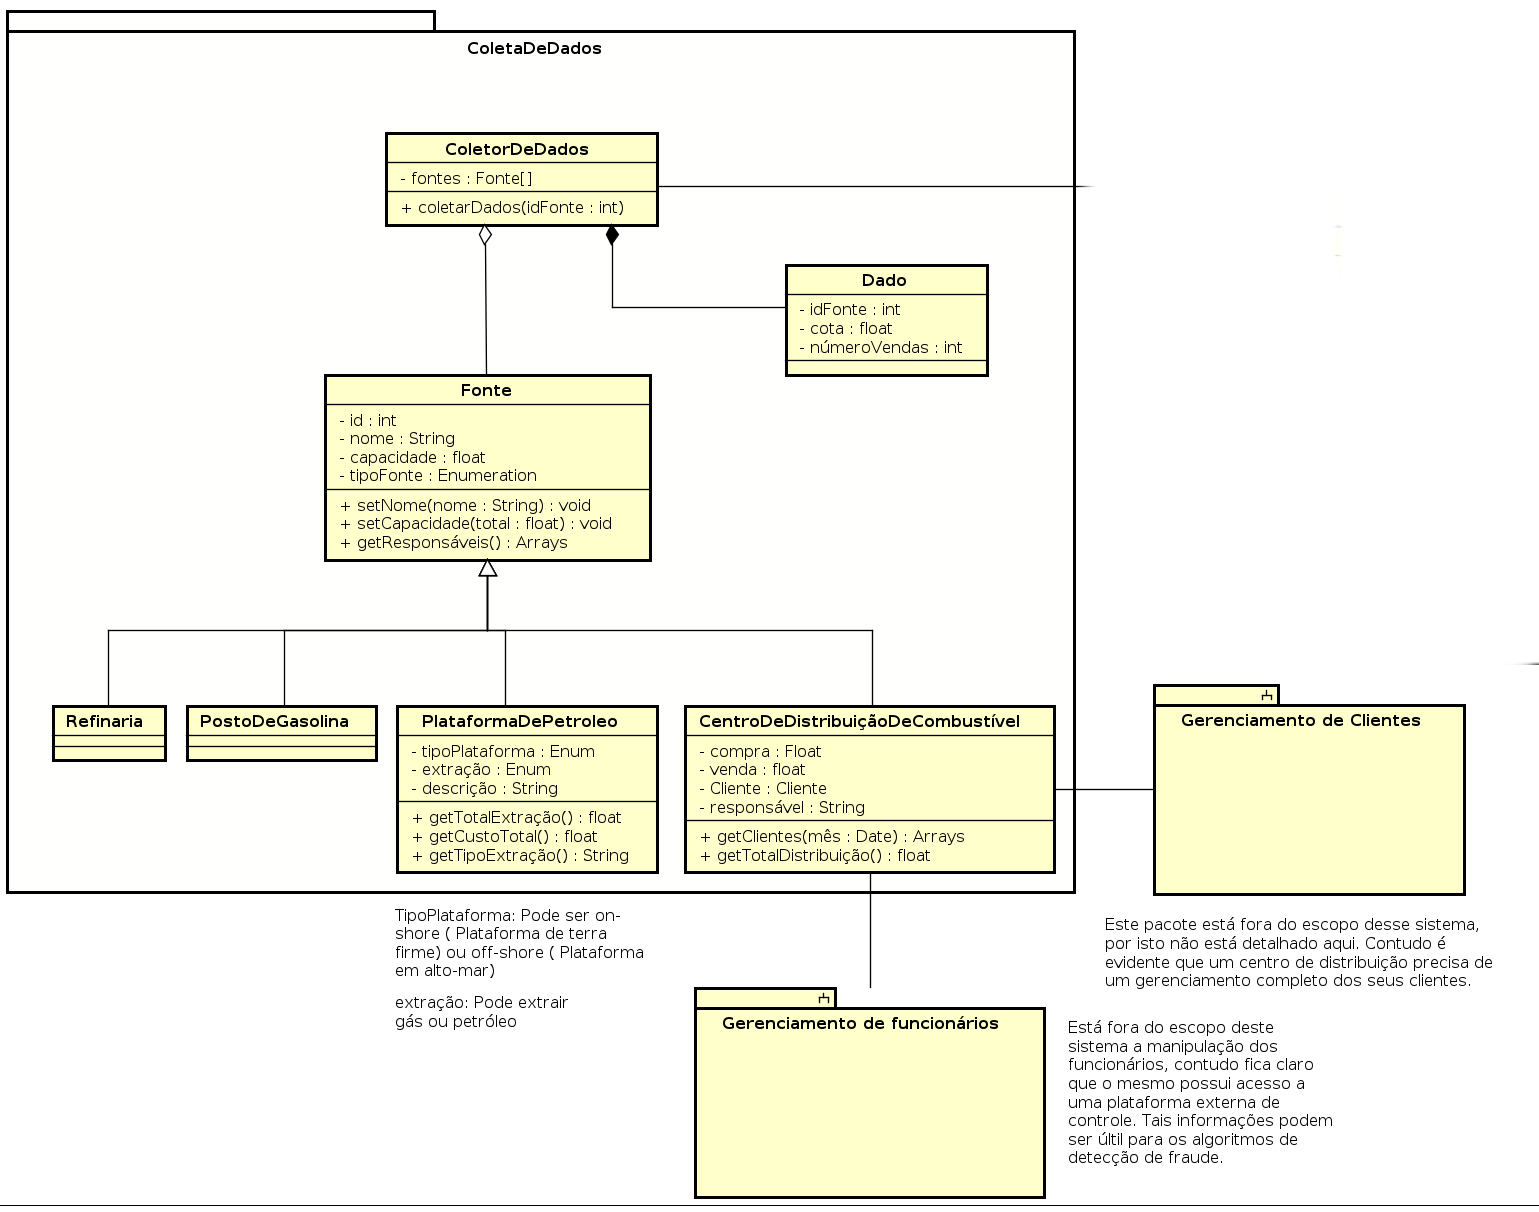
\includegraphics[width=1\textwidth, keepaspectratio=true]{images/coleta.png}
  \caption {Módulo de coleta de dados}
  \label {coleta}
\end{figure}

\subsection{Módulo do Motor de Inferência}

Este módulo recebe os dados coletados e executa os algoritmos de detecção de fraude.
De acordo com a especificação do sistema, algoritmos diferentes são aplicados de
acordo com a forma, tipo e local de compra. Por isso, aplicamos o padrão de projeto
\emph{Strategy}, o que facilita a inserção de novos algoritmos no projeto. Os que
foram apresentados no diagrama são alguns casos que pensamos ser importantes. \par

Veja a \emph{Figura \ref{motor}} mostrando como este módulo foi planejado.

\begin{figure}[ht]
  \centering
  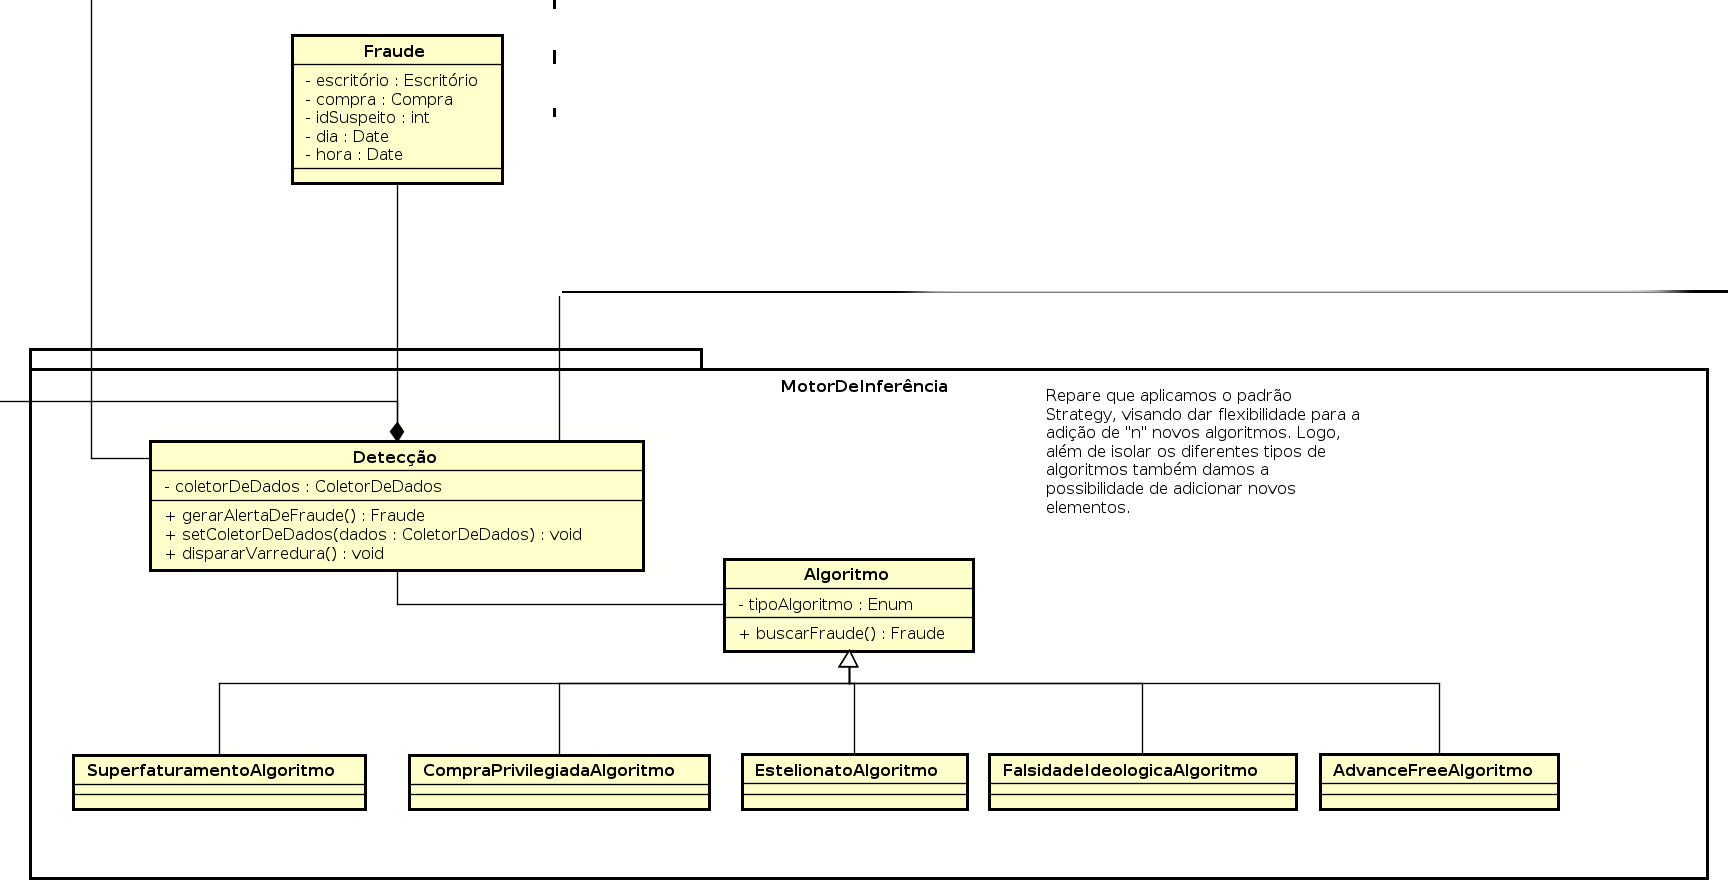
\includegraphics[width=1\textwidth, keepaspectratio=true]{images/motor.png}
  \caption {Módulo do motor de inferência}
  \label {motor}
\end{figure}

\subsection{Módulo de Compras}

Com base nas informações da especificação e em uma pesquisa feita sobre os
conceitos importantes envolvidos nas compras, realizamos a modelagem apresentada
na \emph{Figura \ref{compras}}. Novamente aplicamos o padrão \emph{Strategy}, mas
dessa vez de uma forma mais aimpla, com diferentes interfaces para manipular as
diferentes formas, tipos e locais. \par

\begin{figure}[ht]
  \centering
  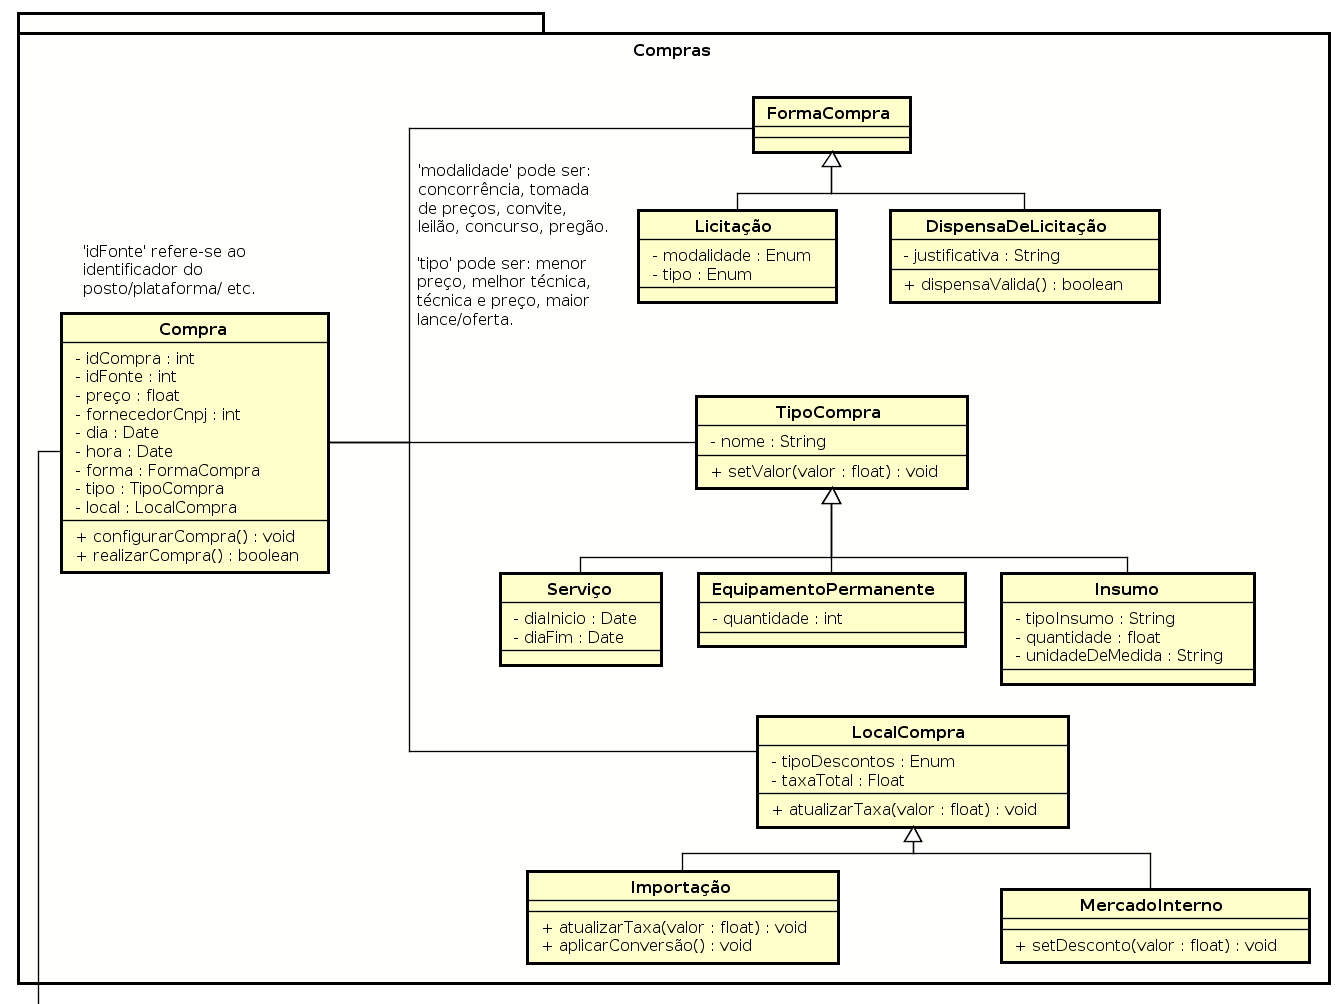
\includegraphics[width=1\textwidth, keepaspectratio=true]{images/compras.png}
  \caption {Módulo de compras}
  \label {compras}
\end{figure}

%------------------------------------------------------------------------
%---------------------- Diagrama de Implantação -------------------------
%------------------------------------------------------------------------

\newpage
\section{Diagrama de Implantação}

\begin{figure}[ht]
  \centering
  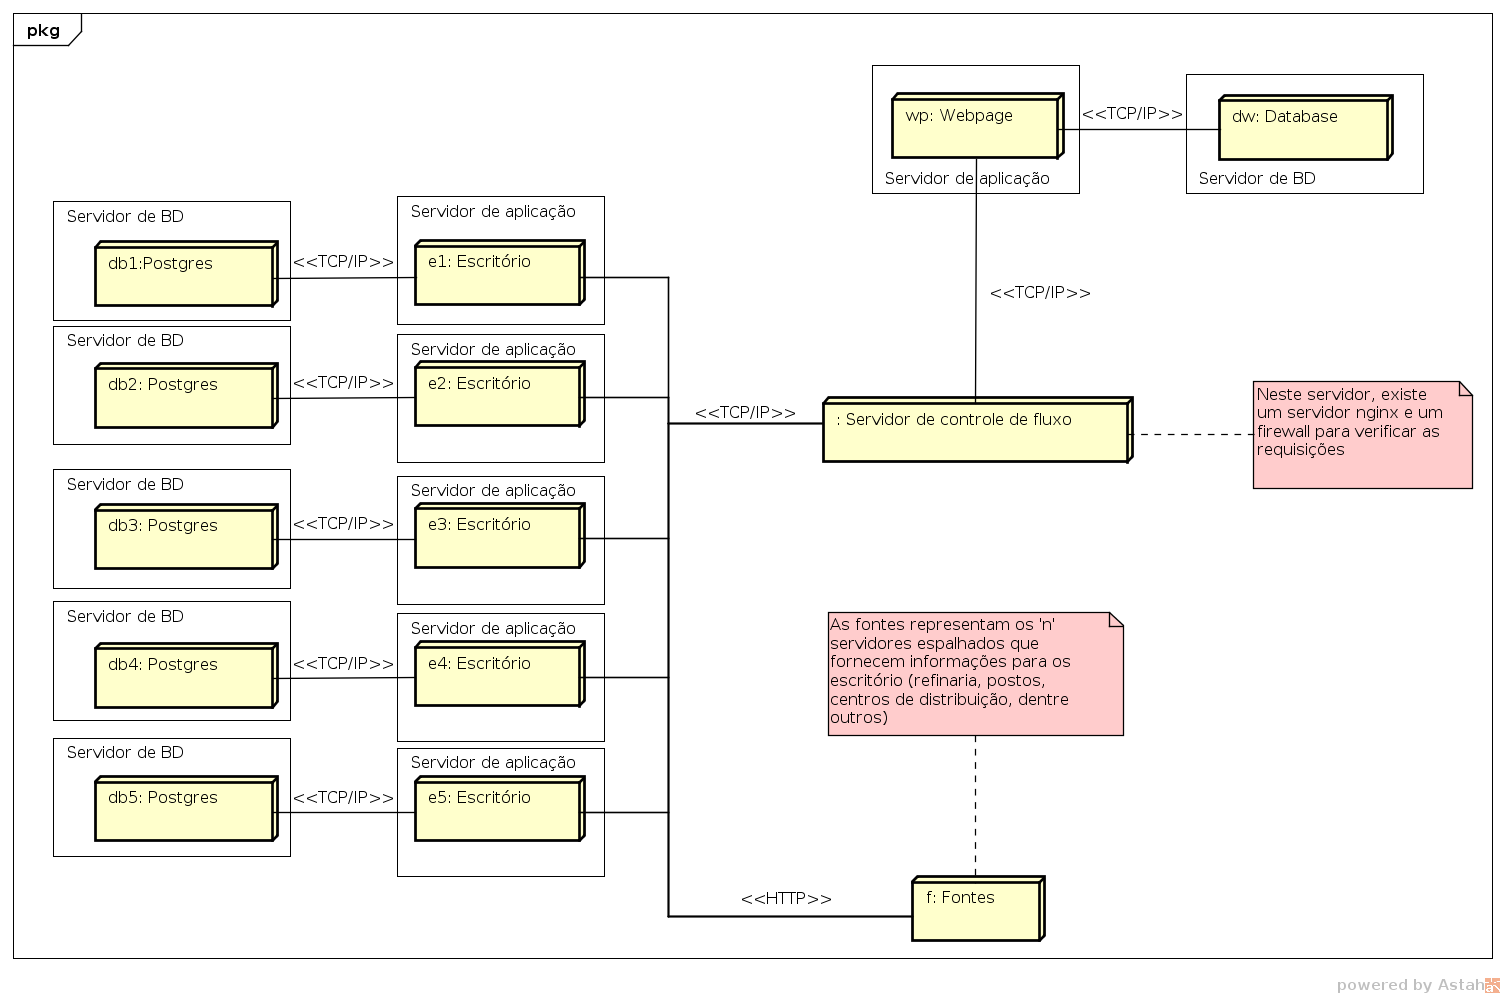
\includegraphics[width=1\textwidth, keepaspectratio=true]{images/implantacao.png}
  \caption {Diagrama de Implantação}
  \label {di}
\end{figure}

O último diagrama criado foi o de implantação (veja a \emph{Figura \ref{di}}). \par

Note que os 5 escritórios foram modelados de maneira similar (um servidor de
aplicação e um servidor de banco de dados), mas todos separados, ilustrando a
natureza distribuída do sistema. \par

O sistema web que publica as possíveis fraudes foi colocado à parte, conectado
aos 5 escritórios. Por uma questão de controle, adicionamos uma camada extra
que recebe e trata as requisições, passando-as para a aplicação web em seguida. \par

As diferentes fontes foram conectadas via HTTP, uma vez que elas estão
localizadas em diferentes pontos e podem ter implementações diferentes.
A utilização do protocolo em questão facilita a distribuição do sitema.

% -----------------------------------------------------------------------

\end{document}
